\section{Typography}
\subsection{Figures and tables}
The thesis should include figures and tables to support the text. They should be placed in the following manner as is automatically done when following the model of this \LaTeX\ template:

\begin{itemize}
    \setlength\itemsep{0pt}
    \setlength\parskip{0pt}
    \item In tables, the heading has to be placed above the table. The
      table heading should not end in a full stop. The permission to
      publish a table copied from another source has to be mentioned
      as part of the table heading. Many publishers inform the correct
      form to write this permission when such a permission has been
      granted. The table must be in text format – not an image.
    \item If necessary, the caption should be separated from the
      figure with a single line spacing for reasons of clarity. A
      figure and a short caption are centered. However, a caption
      spanning multiple lines is justified at both ends. The necessary
      references are included in the figure captions. Copyright
      information is also added to the end of the caption. The
      permission to publish a figure copied form another source has to
      be mentioned as part of the figure text. Many publishers inform
      the correct form to write this permission when such a permission
      has been granted.  The copyright issues and citation practices
      of images are further discussed in~\secref{copyright}.
    \item Do not start a chapter with a figure, but embed it in the
      text content. A figure is supposed to always appear in the text
      after its reference. If there is not enough space for the figure
      directly after the first reference, the word processor moves the
      figure automatically to the next page. In such case, the figure
      can be moved forward so that text originally after the figure
      fills the empty space. However, a figure should always be placed
      in the same chapter---hence sometimes empty space at the bottom
      of some chapters cannot be avoided (the same rules applies for
      the tables).
\end{itemize}

\subsubsection{Formatting the figure captions}
Figures, tables and appendices are a part of the written
presentation. All these need to be referenced to in the text body,
preferably before the figure is placed in the text---i.e., first the
referring text, then the figure or table. Figures and tables have a
running number through the document---or chapter wise, if there are
plenty of figures.

\figref{fig:work_packages} serves as an example of a figure and a text
referring to it. Figure captions are below the figure, and the caption
text ends with a full stop. A short caption is centered, while a long
caption extending to a several lines is justified on both sides. 

If no outside source is referred to in the caption, it is assumed that
the author of the thesis is also the author and copyright owner (not necessarily the author) of the figure, and the license of the figure is the same as the document (Default: \enquote{All rights reserved}). This is discussed further in Section~\secref{copyright}.

Figures and tables should be given an alternative text that summarises
the information they contain for the reader. This is discussed further
in~\secref{accessibility}. Unfortunately support for this in
\LaTeX\ is still work in progress, and the alternative text will
currently not end up in the final PDF. A suitable alt text
for~\figref{fig:work_packages} could be:

\begin{quote}
  Diagram showing interactions between work packages WP1 to WP5, all inside WP6, which is itself inside WP7. WP3 (left) sends outputs to WP1, WP2, and WP4. WP1 and WP2 are bidirectionally linked. WP1, WP2, and WP4 send outputs to WP5 (right). A curved arrow shows WP3 also directly feeding into WP5''.
\end{quote} 

The final thesis will be published as a PDF/A file, and this LaTeX
template produces files in that format directly (There is no need to
use Muuntaja). Be sure to remove all transparency in your source
images to ensure the end result is also compliant. Instructions on doing this are included with the thesis template.

% Pictures in .pdf, .png or .jpg. No need to specify the extension.
% Transparent images are not allowed with PDF/A.
% With ImageMagick transparency can be removed with
% convert image.png -background white -alpha remove -alpha off image_nobg.png
% This restriction also affects PDF images, as a first step try to make the PDF
% image PDF/A:
% gs -dPDFA -dBATCH -dNOPAUSE -sColorConversionStrategy=UseDeviceIndependentColor -sDEVICE=pdfwrite -dPDFACompatibilityPolicy=2 -sOutputFile=output.pdf input.pdf 
\begin{figure}[ht]
  \begin{center}
    \includegraphics*[width=0.7\textwidth]{WP}
  \end{center}
  \caption{Connections between work packages (WP). \copyrightstring\ \href{https://creativecommons.org/licenses/by/4.0/}{CC BY 4.0}.}
  \alt{Diagram showing interactions between work packages WP1 to WP5, all inside WP6, which is itself inside WP7. WP3 (left) sends outputs to WP1, WP2, and WP4. WP1 and WP2 are bidirectionally linked. WP1, WP2, and WP4 send outputs to WP5 (right). A curved arrow shows WP3 also directly feeding into WP5.}
  \label{fig:work_packages}
\end{figure}

\section{Copyright, CC-licenses and the Use of images}
\label{copyright}
Intellectual property rights (IPR) protect works, i.e., the authors
and rights-holders of literary or artistic works that exceed the
threshold of originality. These works include, for instance, texts,
images, music, and computer software code. This section explains the
related issues, especially concerning images, and provides guidelines
for dealing with copyright matters in your thesis.

Your thesis is also a copyrighted work. If no license is explicitly
stated, the license is \enquote{All rights reserved,} meaning it can only be
used in limited ways under copyright law. The Federation of Finnish
Open Science Coordination in Finland and the University of Oulu
recommend publishing theses as open access and under a CC-BY license,
or if warranted, another CC license~\cite{coordination_open_2024}.
CC-BY allows reuse, including commercial use, of your work as long as
the author is credited.

Example copyright pages for your thesis are provided 
with this template. If your license is \enquote{All rights reserved} and
you include all relevant copyright information in the image captions, you can also leave the page out.

Among the various types of works protected by copyright, images present particular challenges and considerations. Images are frequently used to illustrate concepts, present data, or enhance the visual appeal of academic texts. However, their use is subject to specific copyright restrictions, and improper use can lead to legal and ethical issues.
For this reason, figures found on the Internet, for example, may not be freely used in theses without proper permission or licensing. 

According to the copyright enactments, you must always have the
permission from the copyright holder to use their figure in your
work. To summarize: \textbf{Copyright infringement may lead to legal
  actions and penalties, and in those cases the author is
  responsible.} The writer should grow towards to mainly using figures
of his own in the thesis. Often it is necessary to redraw the figure
and cite the original source.

It is good practice to explicitly state the copyright owners and
license for all images in your thesis. This can be done via a blanket
statement on a separate copyright page, or for every image separately
in the caption. All exceptions to the main license of your thesis
(e.g., \enquote{All rights reserved} or \enquote{CC-BY 4.0}) should \textbf{always} be
included in the image captions. If your use of external images is extensive and is a central part of your thesis, you should explicitly mention 
the images on the copyright page, e.g., \enquote{Figure 5 is reproduced from [x] under the provisions of copyright law allowing use with appropriate citation.}
and discuss their use and limitations in publishing your thesis with your thesis supervisor at an early stage.

The starting point is that the figures must be related to the text,
i.e, the text must explain why the figure has been presented. The text
must contain a reference to the figure. Use self-made figures
(drawings, schematics, simulation or measurement result figures,
photographs), if possible.

It is a good practice to mark the photographer in the photos
(e.g. “Photographer first name last name year.”) If you are not the
photographer, ask permission and keep the permission (e.g., email
correspondence) safe. In addition, keep any other licences you have
received, including those under the CC licence, safe. Often
publications under a CC licence mention the CC licence on the front
page and the figure is on page z. Save at least the page explaining
the CC licence from the publication from which you have taken the
photo.

As mentioned, in case the figure has been taken from elsewhere, the
author needs to have a permission from the copyright holder. Usually
this is based on a licence that gives permission to use the work with
some conditions. The most common example would be a CC-BY licence,
such as the one used in \figref{fig:ccbypic}. If the figure is from a
publication you are citing, ”CC-BY 4.0 from [x].” would
 be appropriate.

\begin{figure}[H]
  \begin{center}
    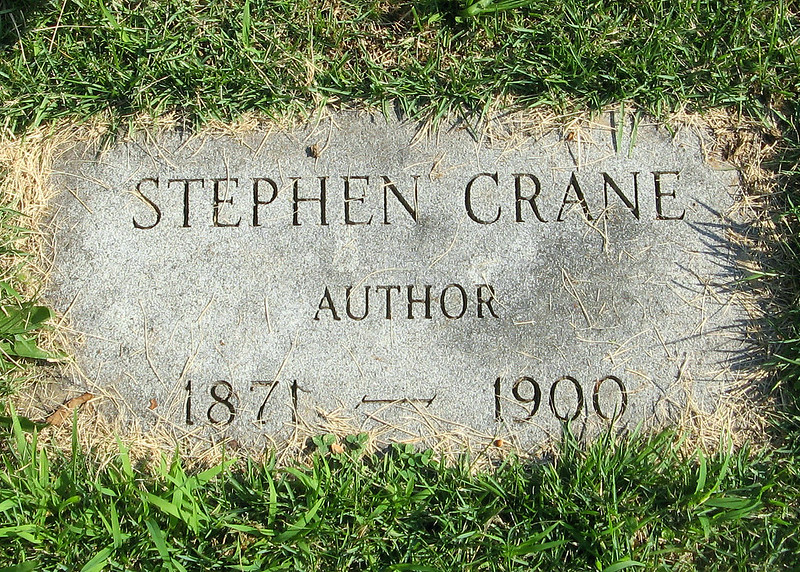
\includegraphics[width=12cm]{Figures/ccby.jpg}
  \end{center}
    \caption{\enquote{\href{https://openverse.org/image/110032f8-1a7a-421f-86b1-88fdfde2e44f }{Stephen Crane, Author, Red Badge of Courage}} by~\href{https://www.flickr.com/photos/tonythemisfit/}{Tony Fischer Photography} is licensed under \href{https://creativecommons.org/licenses/by/2.0/}{CC BY 2.0}.}
    \label{fig:ccbypic}
\end{figure}

If you use figures made by others, you must have permission from the
copyright owner to use the figure. For instance, IEEE and many other
publishers have an automated system for granting permission for
theses. Mark the permission in the caption as requested by the right
holder, e.g., “Reprinted with permission from [x] \textcopyright\ IEEE, 2022.”.

Not all figures exceed the threshold of originality. These include,
for example, scientific diagrams and flowcharts. Good research
practices require that even in this case, the source is cited in the
caption (\enquote{Figure from source [x].}). However, it would be best to ask
for permission or at least redraw the image. Images with a CC license 
are free to use, so long as the terms of use are followed~\cite{about_cc_licenses}. Even then, the
caption must mention the source (article, website, etc.) and that the
image is CC-licensed.

Based on the right to quote, it is possible to take a photocopy,
screenshot or photograph of a work (not the original file) and publish
it, citing the original source in the caption. A critical aspect of
the right to quote is that the use of the image is relevant to the
work, i.e., the image must be related to the subject, and it must be
explained in the text (this applies to all images). Similarly, the
source must be cited in text citations.

Sometimes you may want to use someone else's original image idea as a
basis for your own work. Permission is not required provided that your
work clearly an amply edited version of the original. However, in
accordance with good research practices, the type of modification
(“Modified/Adapted/Redrawn from/Based on/Created using
data from\enquote{) and source }from [x]" must be declared in
the caption. Should you only make minor edits to the original,
separate permission is required. The University of Oulu Acta Oulu
publishing guide~\cite{ronkainen_copyright, ronkainen_tekijanoikeus}
has more details on this topic.

When searching for images through an internet image search, it is not
always easy to find the rights holder from whom to request permission
for use. Hunting for a permit can be a demanding task. The easiest way
is to use images and figures from scientific articles (or with open licenses) as in these the
rights holders are clearly declared.

\section{Accessibility}
\label{accessibility}
Put effort into the accessibility of your Master’s thesis. The
structure of an accessible document is clear, and the wording is as
understandable as possible. Figures and tables should be given an
alternative text that summarises the information they contain for the
reader. Alternative text is especially important in situations where
the reader cannot see the figure or table, for example due to vision
impairment.  More information on accessible Word documents and
archivable PDF files can be found in the texts of the University of
Oulu Campus ICT~\cite{ictaccessibleword,ictwordpdfa}. You can also
read about the accessibility of mathematical equations in the Campus
ICT text~\cite{ictaccessiblemath}.

